While in many cases modeling OCL arithmetic and logic on attributes is straight forward, there are edge cases we must consider.
The reason for this is UML allowing for optional properties: \inlineocl{[0..1] Boolean} and \inlineocl{[0..1] Int}.
For situations where the property is required, we can simply use arithmetic and logic operations.

\subsection{3-valued logic for OCL}
OCL is fundamentally a 4-valued logic, with values: true, false, void, and invalid.
Both Void and invalid behave similarly for the logical operations, and we have chosen to combine them in our encoding.
However invalid expressions can often be statically detected, and stop the interpretation before building the CSP.
OCL\# also collapses OCL to a 3-valued logic using the empty set $\emptyset$ to encode void and invalid expressions. \ytodo{because RFOL}

\begin{table}[!ht]
    \begin{tabular}{c|c|c|c|c|c|c}
    a & b & a and b & a or b & a xor b & a implies b & not a \\ \hline
    2 & 2 & 2       & 2      & 0       & 2           & 0     \\ \hline
    2 & 1 & 1       & 2      & 1       & 1           & 0     \\ \hline
    2 & 0 & 0       & 2      & 2       & 0           & 0     \\ \hline
    1 & 2 & 1       & 2      & 1       & 2           & 1     \\ \hline
    1 & 1 & 1       & 1      & 1       & 1           & 1     \\ \hline
    1 & 0 & 0       & 1      & 1       & 1           & 1     \\ \hline
    0 & 2 & 0       & 2      & 2       & 2           & 2     \\ \hline
    0 & 1 & 0       & 1      & 1       & 1           & 2     \\ \hline
    0 & 0 & 0       & 0      & 0       & 2           & 2     
    \end{tabular}
\end{table}
In this table we find the semantics for boolean operations in OCL, combining both invalid and void into \textit{maybe}.
For this table we have chosen $\top$=2, \textit{maybe}=1 $\bot$=0.
The semantics for these logical operations encoded with integers can be simply modeled with integer operations:
\begin{itemize}
    \item $\neg a \equiv 2-a$
    \item $a \wedge b \equiv min(a,b)$
    \item $a \vee b \equiv max(a,b)$
    \item $a \rightarrow b \equiv max(2-a,b)$
    \item $a \oplus b \equiv min(2-min(a,b),max(a,b))$
\end{itemize}
We can see these models employ $min$ and $max$ as $and$ and $or$, and $\top -x$ for not, and model \textit{implication} and \textit{the exclusive or} on top:
\begin{itemize}
    \item $a \rightarrow b \equiv (\neg a \vee b)$
    \item $a \oplus b \equiv (\neg(a \wedge b) \wedge (a \vee b))$
\end{itemize}

\subsection{Property encoding to 3-valued logic for optional Booleans}
\begin{figure}[!ht]
    \centering
    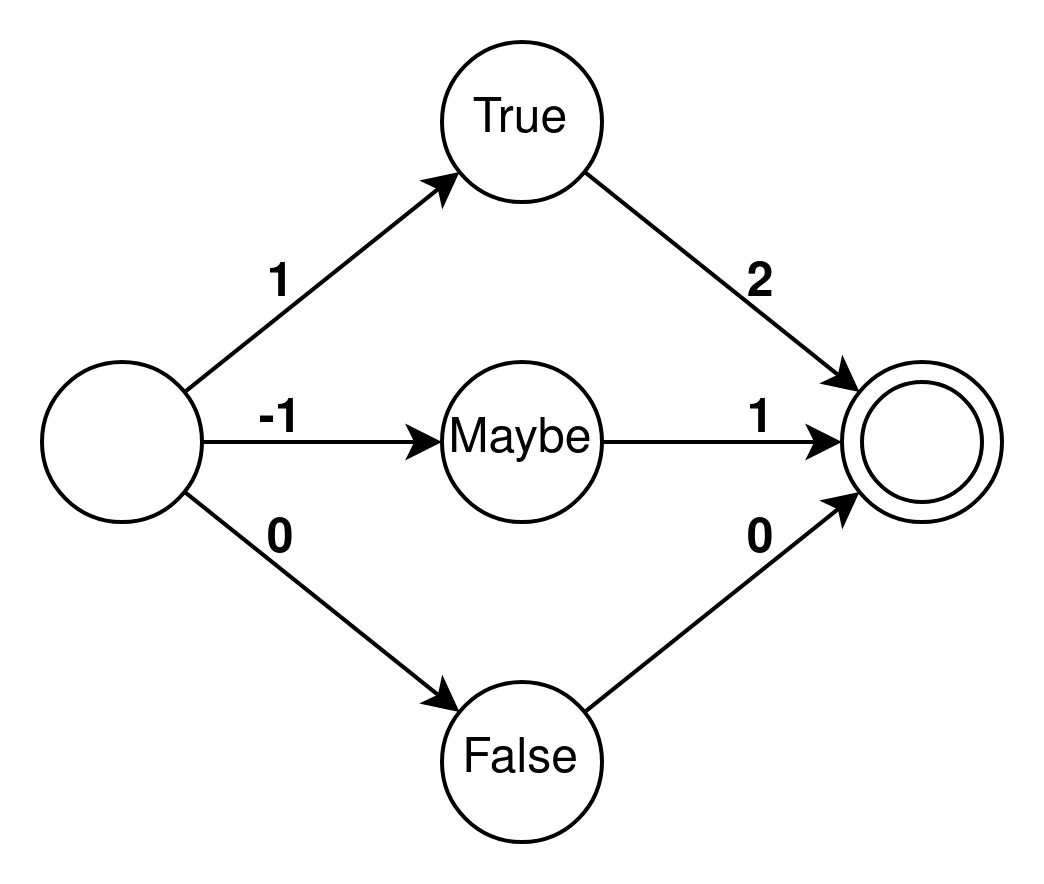
\includegraphics[trim={0 30 0 0},width=0.5\linewidth]{Contributions/OCLCSP/Operations/figures/negbool2halfboolAFD.png}
    \caption{Part of the tree for \inlineocl{src.forall(a,b,c| (a<b and b<c) implies (a+b=c+c))}}
    \label{fig:forallexample}
\end{figure}
In our base encoding for properties, True equals 1, False equals 0, and no information is -1.
We could implement a different encoding for booleans, or simply convert from one encoding to the other using an regular expression constraint based on the AFD here.

\subsection{Operations with Optional Integers}
In the OCL Specification: \textit{The interpretation of operations is considered strict [...]. Hence, an
invalid or null argument value causes an invalid operation result. This ensures the propagation of error conditions.}
This means expressions such as \inlineocl{2 + null} are \textit{invalid}, and generally invalidate the whole model.


To follow the specification and and only handle valid OCL, we can fail by making adding a contradiction to the constraint model, essentially adding \texit{AND False} appropriately.

Taking addition as an example: $x+y=z$, becomes $x+y=z \wedge x \neq d \wedge y \neq d$, to fail because invalid expression: 2 + d = False. In this case: models with data and solver configurations forcing an absence will be invalid and the will be no solution to the CSP, otherwise it will populate all the attributes with values.

However, we can also relax the arithmetic. 
If we didn't want to force the presence of attributes or fail, and wanted to maybe ignore operations on absent values, we can exchange the d value of a variable with another.
For instance $x+y=z$, becomes $$x'+y'=z \wedge (x=d => x'=0) \wedge (x \neq d => x'=x) \wedge (y=d => y'=0) \wedge (y \neq d => y'=y)$$
Here, if either $x$ or $y$ are null, we replace their value with 0 in $x'$ and $y'$, skipping the addition.
We could always interpret null as 0, or choose an interpretation which skips the operations, such as 1 in multiplication, \textit{infinity} in \textit{less than}, etc.. 
% Summing over collection similarly 

\ytodo{OCL\# : in OCL- there is no invalid or null, and arithmetic isn't done with missing values? Check this.}